\chapter{Geometrical Optics}

\section{Aspherical Surface}

\begin{figure}[H]
  \centering
  \begin{subfigure}{.25\textwidth}
    \centering
    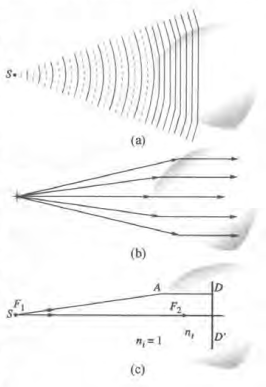
\includegraphics[width=\linewidth]{figures/hyperbolic-surf.png}
  \end{subfigure}
  \begin{subfigure}{.65\textwidth}
    \centering
    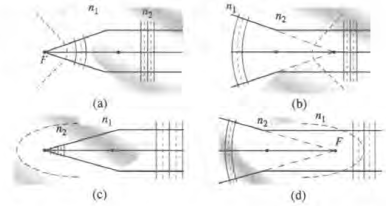
\includegraphics[width=\linewidth]{figures/ellipsoidal-surf.png}
  \end{subfigure}
\end{figure}

\section{Refraction at a Spherical Interface}

\begin{figure}[H]
  \centering
  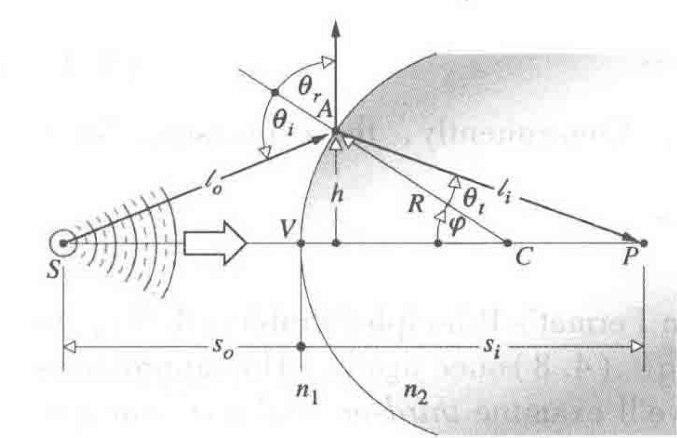
\includegraphics[width=0.5\linewidth]{figures/Refraction-at-a-Spherical-Interface}
\end{figure}

\begin{equation*}
  \begin{aligned}
    \dfrac{n_1}{s_o} + \dfrac{n_2}{s_i} = \dfrac{n_2 - n_1}{R} = \Phi 
  \end{aligned}
  \quad \Rightarrow \quad
  \left\{
  \begin{aligned}
    f_0 = \dfrac{n_1}{n_2 - n_1} R \quad\quad (s_i = \infty) \\
    f_i = \dfrac{n_2}{n_2 - n_1} R \quad\quad (s_o = \infty)  
  \end{aligned}
  \right.
\end{equation*}

\begin{figure}[H]
  \centering
  \begin{subfigure}{.3\textwidth}
    \centering
    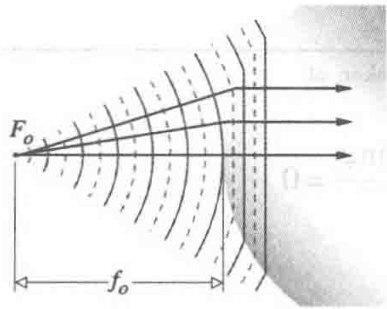
\includegraphics[width=\linewidth]{figures/Refraction-at-a-Spherical-Interface-1.jpg}
  \end{subfigure}
  \hspace{2cm}
  \begin{subfigure}{.4\textwidth}
    \centering
    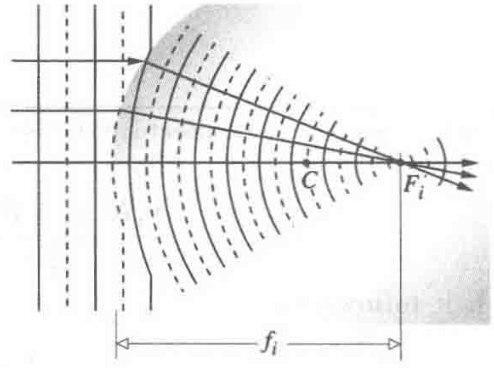
\includegraphics[width=\linewidth]{figures/Refraction-at-a-Spherical-Interface-2.jpg}
  \end{subfigure}
\end{figure}

\section{Lenses}

\begin{figure}[H]
  \centering
  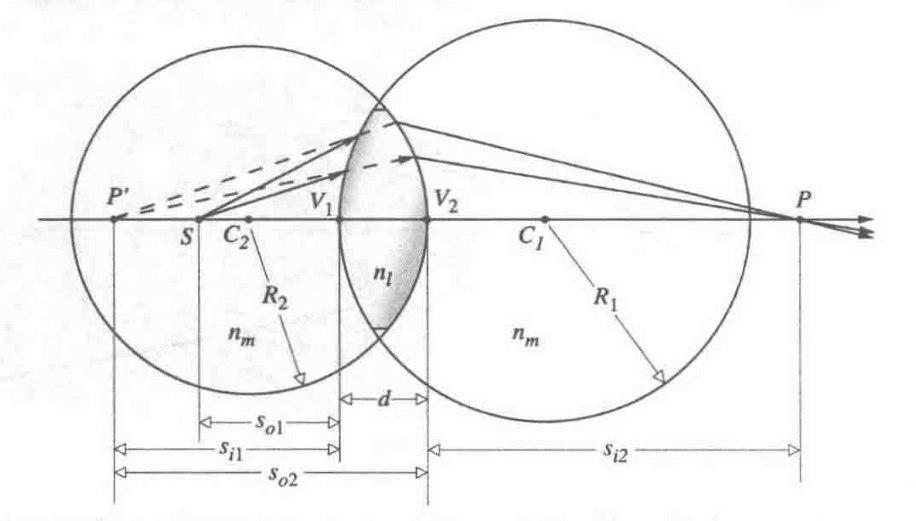
\includegraphics[width=0.5\linewidth]{figures/Thin-Lens.jpg}
\end{figure}

\begin{equation*}
  \begin{aligned}
    \dfrac{n_m}{s_{o1}} + \dfrac{n_m}{s_{i2}} = \left( n_l - n_m \right) \left( \dfrac{1}{R_1} - \dfrac{1}{R_2}   \right) + \dfrac{n_l d}{\left( s_{i1} - d \right) s_{i1}} 
  \end{aligned}
\end{equation*}

For lenses in the air, where $n_m = 1$

\begin{equation*}
  \begin{aligned}
    \dfrac{1}{s_{o1}} + \dfrac{1}{s_{i2}} = \left( n_l - 1 \right) \left( \dfrac{1}{R_1} - \dfrac{1}{R_2}   \right) + \dfrac{n_l d}{\left( s_{i1} - d \right) s_{i1}} 
  \end{aligned}
\end{equation*}

For thin lenses, $d \approx 0$

\begin{equation*}
  \begin{aligned}
    \dfrac{1}{s_{o1}} + \dfrac{1}{s_{i2}} = \left( n_l - 1 \right) \left( \dfrac{1}{R_1} - \dfrac{1}{R_2}   \right) = \dfrac{1}{f} 
  \end{aligned}
\end{equation*}

Which is the Lensmaker's Formula.

\section{Magnification}

\begin{figure}[H]
  \centering
  \begin{subfigure}{.45\textwidth}
    \centering
      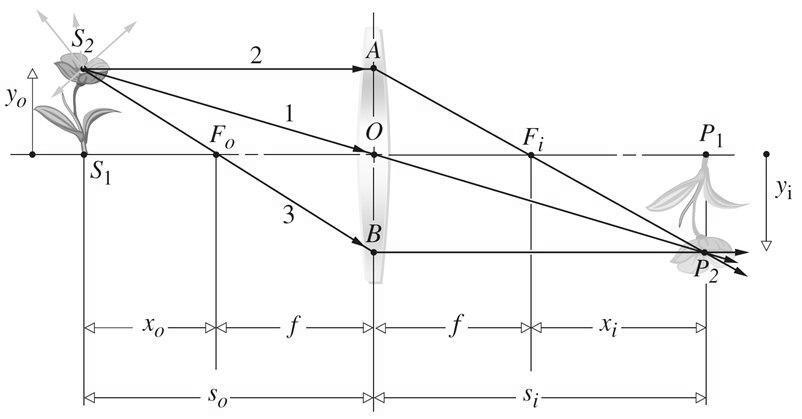
\includegraphics[width=\linewidth]{figures/Magnification-transverse.jpg}
  \end{subfigure}
  \begin{subfigure}{.45\textwidth}
    \centering
      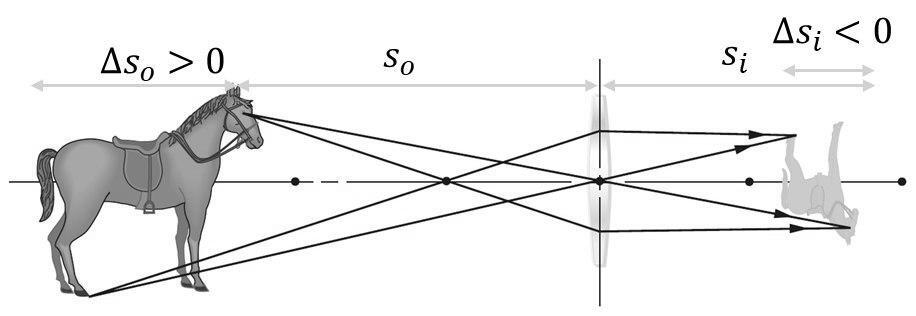
\includegraphics[width=\linewidth]{figures/Magnification-longitudinal.jpg}
  \end{subfigure}
\end{figure}

\begin{equation*}
  \left\{
  \begin{aligned}
    \dfrac{y_o}{|y_i|} = \dfrac{f}{x_i} \\
    \dfrac{|y_i|}{y_o} = \dfrac{f}{x_o}  
  \end{aligned}
  \right.
  \quad \Rightarrow \quad
  \begin{aligned}
    x_o x_i = f^2 \quad\quad \left( \text{Newton's formula} \right)
  \end{aligned}
\end{equation*}


Transverse Magnification

\begin{equation*}
  \begin{aligned}
    M_T = \dfrac{y_i}{|y_o|} = - \dfrac{s_o}{s_i} = - \dfrac{f}{x_o} = - \dfrac{x_i}{f}  
  \end{aligned}
\end{equation*}

Longitudinal Magnification

\begin{equation*}
  \begin{aligned}
    M_L = \dfrac{\md x_i}{\md x_o} = \dfrac{\md}{\md x_o} \left( \dfrac{f^2}{x_o}  \right) = - \dfrac{f^2}{x_o^2} = - M_T^2   
  \end{aligned}
\end{equation*}

\section{Mirrors}

\subsection{Aspherical Mirrors}

\begin{figure}[H]
  \centering
  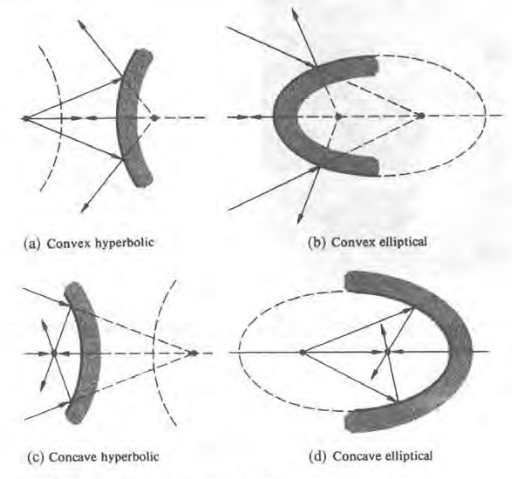
\includegraphics[width=0.7\linewidth]{figures/aspherical-mirror.png}
\end{figure}

Precise aspheric surface are difficult and expensive to fabricate.

\subsection{Spherical Mirrors}

The difference between spherical and paraboloidal mirror will be appreciable only if y is large.

\begin{figure}[H]
  \centering
  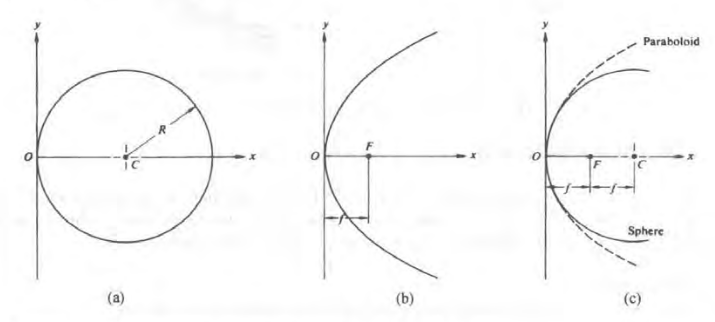
\includegraphics[width=0.7\linewidth]{figures/spherical-aspherical.png}
\end{figure}

\subsubsection{Mirror Formula}

\begin{figure}[H]
  \centering
  \begin{subfigure}{.45\textwidth}
    \centering
    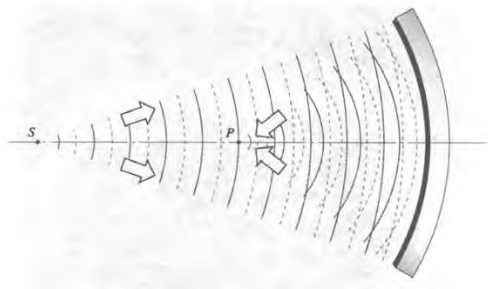
\includegraphics[width=\linewidth]{figures/mirror-formula-0.png}
  \end{subfigure}
  \begin{subfigure}{.45\textwidth}
    \centering
    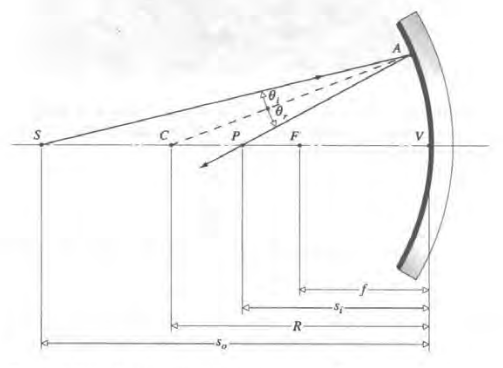
\includegraphics[width=\linewidth]{figures/mirror-formula-1.png}
  \end{subfigure}
\end{figure}

\begin{equation*}
  \begin{aligned}
    \dfrac{\overline{SC}}{\overline{SA}} = \dfrac{\overline{CP}}{\overline{PA}}  
  \end{aligned}
  \quad + \quad
  \left\{
  \begin{aligned}
    \overline{SC} &= \phantom{-} s_o - \left| R \right| = \phantom{-(} s_o + R \phantom{)} \\ 
    \overline{CP} &= - s_i + \left| R \right| = -  \left( s_i + R \right) \\
    \overline{SA} &= s_o \\
    \overline{PA} &= s_i
  \end{aligned}
  \right.
  \quad \Rightarrow \quad
  \begin{aligned}
    \dfrac{s_o + R}{s_o} = - \dfrac{s_i + R}{s_i}  
  \end{aligned}
  \quad \Rightarrow \quad
  \begin{aligned}
    \dfrac{1}{s_o} + \dfrac{1}{s_i} = - \dfrac{2}{R}   
  \end{aligned}
\end{equation*}

\begin{equation*}
  \left\{
  \begin{aligned}
    s_o = \infty \quad \Rightarrow \quad s_i = f = - R / 2 \\
    s_i = \infty \quad \Rightarrow \quad s_o = f = - R / 2 
  \end{aligned}
  \right.
  \quad \Rightarrow \quad 
  \left\{
  \begin{aligned}
    s_o = 2f \quad \Rightarrow \quad s_i = 2f \\
    s_o = \phantom{1} f \quad \Rightarrow \quad s_i = \infty \\
    s_i = \phantom{1} f \quad \Rightarrow \quad s_o = \infty
  \end{aligned}
  \right.
\end{equation*}

\section{Prism}

\begin{figure}[H]
  \centering
  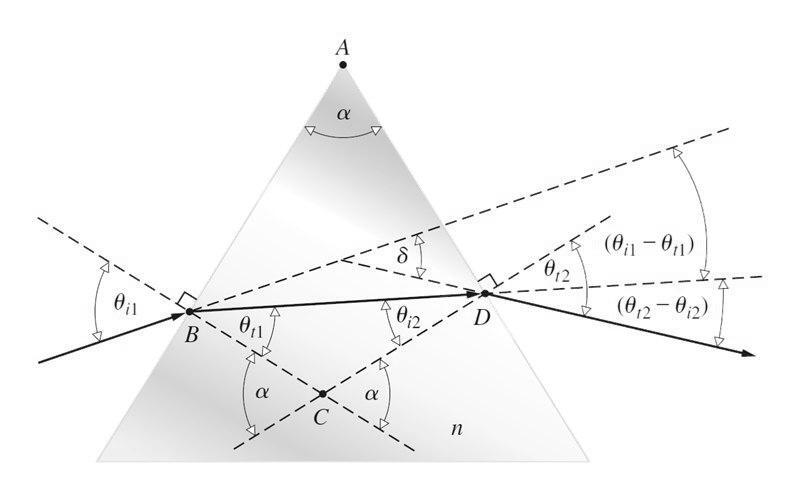
\includegraphics[width=0.5\linewidth]{figures/Prism}
\end{figure}

\begin{equation*}
  \left\{
  \begin{aligned}
    \delta &= \left( \theta_{i1} - \theta_{t1} \right) + \left( \theta_{t2} - \theta_{i2} \right) \\
    \alpha &= \theta_{t1} + \theta_{i2}
  \end{aligned}
  \right.
  \quad \Rightarrow \quad 
  \begin{aligned}
    \delta &= \theta_{i1} + \theta_{t2} - \alpha
  \end{aligned}
\end{equation*}

\begin{equation*}
  \begin{aligned}
    \theta_{t2} &= \sin^{-1} \left( n \sin \theta_{i2} \right) 
    = \sin^{-1} \left[ n \sin \left( \alpha - \theta_{t1} \right) \right] 
    = \sin^{-1} \left[ n \left( \sin \alpha \cos \theta_{t1} - \cos \alpha \sin \theta_{t1} \right) \right] \\
    &= \sin^{-1} \left[ n \left( \sin \alpha \sqrt{1 - \sin^2 \theta_{t1}} - \cos \alpha \sin \theta_{t1} \right) \right] 
    = \sin^{-1} \left[ \sin \alpha \sqrt{n^2 - \sin^2 \theta_{i1}} - \cos \alpha \sin \theta_{i1} \right] \\
  \end{aligned}
\end{equation*}
  
\begin{equation*}
  \begin{aligned}
    \delta &= \theta_{i1} + \sin^{-1} \left[ \sin \alpha \sqrt{n^2 - \sin^2 \theta_{i1}} - \cos \alpha \sin \theta_{i1} \right] - \alpha
  \end{aligned}
\end{equation*}

Minimum deviation:

\begin{equation*}
  \left\{
  \begin{aligned}
    & \dfrac{\md \delta}{\md \theta_{i1}} = 0 \quad \Rightarrow \quad 1 + \dfrac{\md \theta_{t2}}{\md \theta_{i1}} = 0 \quad \Rightarrow \quad \md \theta_{i1} = - \md \theta_{t2} \\
    & \md \alpha = 0 \quad \Rightarrow \quad \md \left( \theta_{t1} + \theta_{i2} \right) = 0 \quad \Rightarrow \quad \md \theta_{t1} = - \md \theta_{i2} \\
    & \sin \theta_{i1} = n \sin \theta_{t1} \quad \Rightarrow \quad \cos \theta_{i1}\md \theta_{i1} = n \cos \theta_{t1} \md \theta_{t1} \\
    & \sin \theta_{t2} = n \sin \theta_{i2} \quad \Rightarrow \quad \cos \theta_{t2}\md \theta_{t2} = n \cos \theta_{i2} \md \theta_{i2}
  \end{aligned}
  \right.
  \quad \Rightarrow \quad 
  \begin{aligned}
    \dfrac{\cos \theta_{i1}}{\cos \theta_{t2}} = \dfrac{\cos \theta_{t1}}{\cos \theta_{i2}}  
  \end{aligned}
\end{equation*}

$\Rightarrow $

\begin{equation*}
  \begin{aligned}
    \dfrac{1 - \sin^2 \theta_{i1}}{1 - \sin^2 \theta_{t2}} = \dfrac{1 - n^2 \sin^2 \theta_{i1}}{1 - n^2 \sin^2 \theta_{t2}}  
  \end{aligned}
  \quad \Rightarrow \quad 
  \begin{aligned}
    \theta_{i1} = \theta_{t2}
  \end{aligned}
\end{equation*}

This means that the ray for which the deviation is a minimum traverses the prism symmetrically.

\begin{equation*}
  \begin{aligned}
    \theta_{t1} = \theta_{i2} = \alpha / 2 \quad\quad \theta_{i1} = \theta_{t2} = \dfrac{\delta_m + \alpha}{2} \quad\quad n = \dfrac{\sin \left[ \left( \delta_m + \alpha \right) / 2 \right]}{\sin \alpha / 2}  
  \end{aligned}
\end{equation*}

%%% Local Variables:
%%% mode: latex
%%% TeX-master: "Optics"
%%% End:
